``Esta encuesta se enmarca dentro de una tesis doctoral del Instituto de Investigación del Automóvil Francisco Aparicio Izquierdo (Universidad Politécnica de Madrid) sobre la toma de decisiones en la conducción de los vehículos autónomos. El objetivo es valorar qué variables humanas se consideran más importantes a la hora de conducir, con el fin de estudiar posibles mejoras en los algoritmos de los vehículos autónomos, y permitir un tráfico mixto más fluido y natural.

Las siguientes preguntas se ubican siempre en una carretera interurbana, generalmente autovía o autopista, donde la velocidad máxima son 120 km/h. Su vehículo es siempre el coche azul. El trayecto no requiere más que seguir en línea recta, sin cambio de ruta. 
Los resultados son completamente anónimos.''


1. Me gusta ir a velocidad constante
\vspace{-10pt}
\begin{table}[h]
\centering
\begin{tabular}{|c|c|c|c|c|}
\hline
Nunca o casi nunca & Pocas veces & A veces & Muchas veces & Siempre o casi siempre \\ \hline
\end{tabular}
\end{table}

2. Me gusta pisar el acelerador 
\vspace{-10pt}
\begin{table}[h]
\centering
\begin{tabular}{|c|c|c|c|c|}
\hline
Nunca o casi nunca & Pocas veces & A veces & Muchas veces & Siempre o casi siempre \\ \hline
\end{tabular}
\end{table}

3. Si el vehículo de delante va más despacio que yo y me obliga a frenar, le adelanto para mantener una velocidad constante  
\vspace{-10pt}
\begin{table}[h]
\centering
\begin{tabular}{|c|c|c|c|c|}
\hline
Nunca o casi nunca & Pocas veces & A veces & Muchas veces & Siempre o casi siempre \\ \hline
\end{tabular}
\end{table}
\newpage

4. Si el vehículo A va muy deprisa, me espero a que adelante para realizar la maniobra de adelantamiento
\begin{figure}[h]
    \centering
    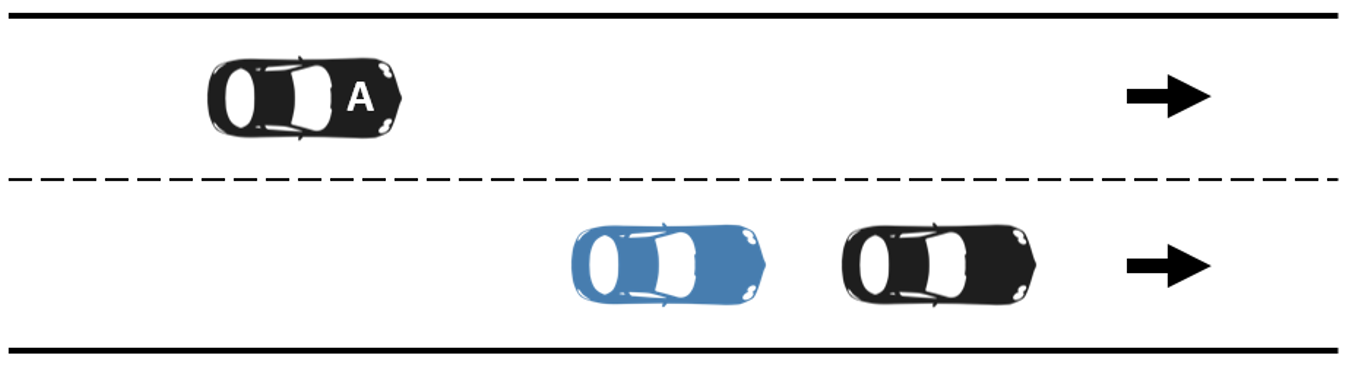
\includegraphics[width=14cm]
    {figures/B1.png}
\end{figure}
\vspace{-10pt}
\begin{table}[h]
\centering
\begin{tabular}{|c|c|c|c|c|}
\hline
Nunca o casi nunca & Pocas veces & A veces & Muchas veces & Siempre o casi siempre \\ \hline
\end{tabular}
\end{table}

5. En un adelantamiento, espero hasta el último momento para adelantar al vehículo de delante, apurando la distancia  
\vspace{-10pt}
\begin{table}[h]
\centering
\begin{tabular}{|c|c|c|c|c|}
\hline
Nunca o casi nunca & Pocas veces & A veces & Muchas veces & Siempre o casi siempre \\ \hline
\end{tabular}
\end{table}

6. En una retención sigo a mi velocidad y no me importa frenar bruscamente a pocos metros del vehículo de delante 
\vspace{-10pt}
\begin{table}[H]
\centering
\begin{tabular}{|c|c|c|c|c|}
\hline
Nunca o casi nunca & Pocas veces & A veces & Muchas veces & Siempre o casi siempre \\ \hline
\end{tabular}
\end{table}

7. Me incomoda conducir detrás de un vehículo más alto que el mío
\vspace{-10pt}
\begin{table}[H]
\centering
\begin{tabular}{|c|c|c|c|c|}
\hline
Nunca o casi nunca & Pocas veces & A veces & Muchas veces & Siempre o casi siempre \\ \hline
\end{tabular}
\end{table}

8. En una retención, me cambio de carril si los vehículos del carril izquierdo parecen ir a mayor velocidad 
\vspace{-10pt}
\begin{table}[H]
\centering
\begin{tabular}{|c|c|c|c|c|}
\hline
Nunca o casi nunca & Pocas veces & A veces & Muchas veces & Siempre o casi siempre \\ \hline
\end{tabular}
\end{table}

9. Cuando tomo decisiones me fijo en lo que hay delante del vehículo que me precede
\vspace{-10pt}
\begin{table}[H]
\centering
\begin{tabular}{|c|c|c|c|c|}
\hline
Nunca o casi nunca & Pocas veces & A veces & Muchas veces & Siempre o casi siempre \\ \hline
\end{tabular}
\end{table}

10. Si en la siguiente situación el vehículo A manifiesta sus intenciones de cambiarse de carril, freno aunque suponga hacerlo de una manera brusca 
\begin{figure}[h]
    \centering
    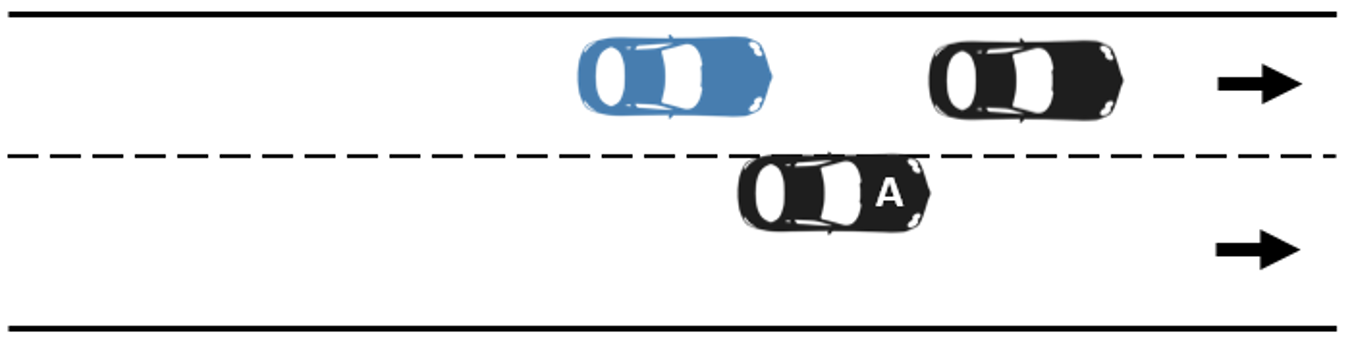
\includegraphics[width=14cm]
    {figures/B2.png}
\end{figure}
\vspace{-10pt}
\begin{table}[h]
\centering
\begin{tabular}{|c|c|c|c|c|}
\hline
Nunca o casi nunca & Pocas veces & A veces & Muchas veces & Siempre o casi siempre \\ \hline
\end{tabular}
\end{table}

11. Adelanto automáticamente si el vehículo de delante es un vehículo pesado o de gran altura, y aunque circule a la velocidad máxima de la vía
\vspace{-10pt}
\begin{table}[h]
\centering
\begin{tabular}{|c|c|c|c|c|}
\hline
Nunca o casi nunca & Pocas veces & A veces & Muchas veces & Siempre o casi siempre \\ \hline
\end{tabular}
\end{table}

12. Prefiero ir a la velocidad máxima de la vía, aunque implique estar demasiado cerca del coche de delante
\vspace{-10pt}
\begin{table}[H]
\centering
\begin{tabular}{|c|c|c|c|c|}
\hline
Nunca o casi nunca & Pocas veces & A veces & Muchas veces & Siempre o casi siempre \\ \hline
\end{tabular}
\end{table}

13. Si hay mucho tráfico y quiero cambiar de carril, no fuerzo el hueco en el carril izquierdo
\vspace{-10pt}
\begin{table}[H]
\centering
\begin{tabular}{|c|c|c|c|c|}
\hline
Nunca o casi nunca & Pocas veces & A veces & Muchas veces & Siempre o casi siempre \\ \hline
\end{tabular}
\end{table}

14. Si el vehículo de delante es un vehículo pesado o de gran altura prefiero adelantarle, aunque tenga que forzar el hueco en el carril izquierdo
\vspace{-10pt}
\begin{table}[H]
\centering
\begin{tabular}{|c|c|c|c|c|}
\hline
Nunca o casi nunca & Pocas veces & A veces & Muchas veces & Siempre o casi siempre \\ \hline
\end{tabular}
\end{table}

15. Prefiero ir a la velocidad máxima de la vía, aunque tenga que forzar el hueco en el carril izquierdo 
\vspace{-10pt}
\begin{table}[H]
\centering
\begin{tabular}{|c|c|c|c|c|}
\hline
Nunca o casi nunca & Pocas veces & A veces & Muchas veces & Siempre o casi siempre \\ \hline
\end{tabular}
\end{table}
\newpage

16. En un adelantamiento donde el vehículo de delante frena de golpe y el vehículo A va a mucha velocidad, prefiero acelerar al máximo y pasar delante del vehículo A que frenar bruscamente
\begin{figure}[h]
    \centering
    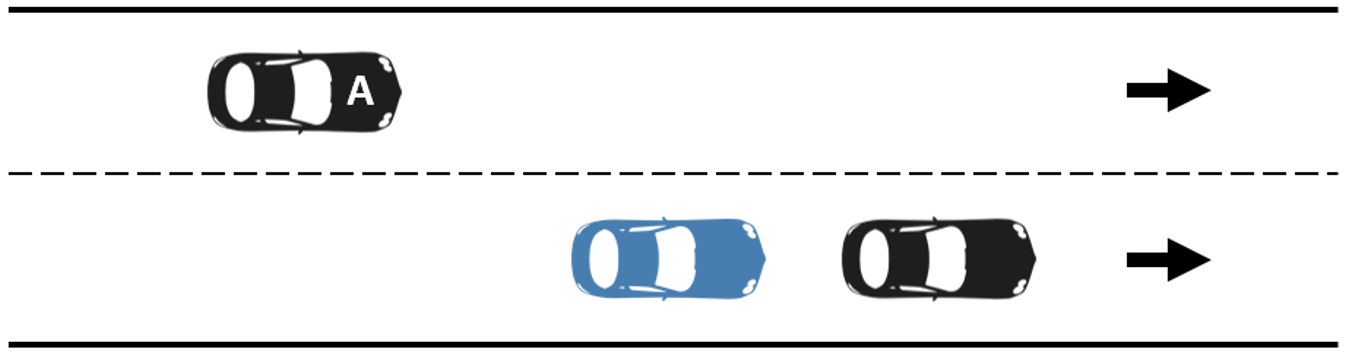
\includegraphics[width=14cm]
    {figures/B3.png}
\end{figure}
\vspace{-10pt}
\begin{table}[h]
\centering
\begin{tabular}{|c|c|c|c|c|}
\hline
Nunca o casi nunca & Pocas veces & A veces & Muchas veces & Siempre o casi siempre \\ \hline
\end{tabular}
\end{table}

17. Si el vehículo de delante es un vehículo pesado o de gran altura prefiero adelantarle, aunque haya mucho tráfico
\vspace{-10pt}
\begin{table}[h]
\centering
\begin{tabular}{|c|c|c|c|c|}
\hline
Nunca o casi nunca & Pocas veces & A veces & Muchas veces & Siempre o casi siempre \\ \hline
\end{tabular}
\end{table}

18. Realizo juicios internos sobre el estilo de conducción de los demás conductores en función del tipo de vehículo, edad y sexo de la persona que conduce
\vspace{-10pt}
\begin{table}[H]
\centering
\begin{tabular}{|c|c|c|c|c|}
\hline
Nunca o casi nunca & Pocas veces & A veces & Muchas veces & Siempre o casi siempre \\ \hline
\end{tabular}
\end{table}

19. Prefiero forzar el hueco entre los vehículos A y B que esperarme a pasar entre los vehículos B y C, aunque perciba que tengo un hueco mayor
\begin{figure}[H]
    \centering
    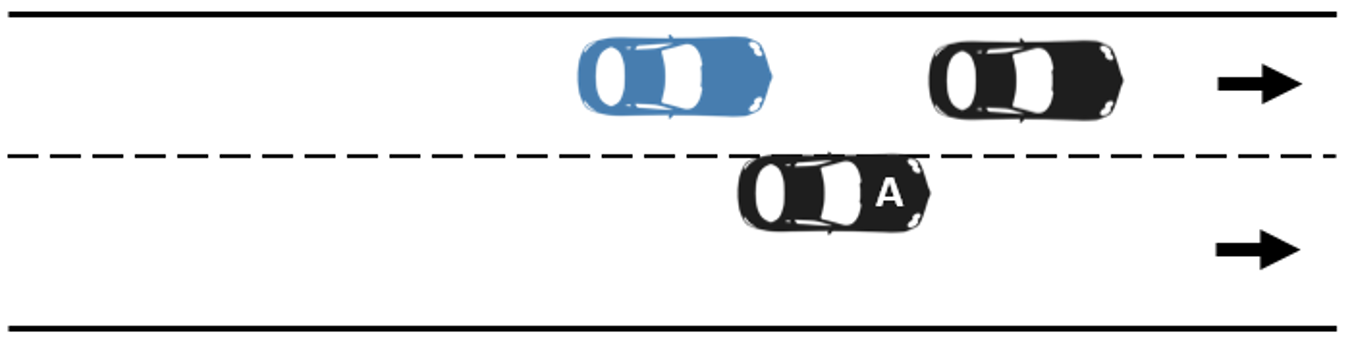
\includegraphics[width=14cm]
    {figures/B2.png}
\end{figure}
\vspace{-10pt}
\begin{table}[H]
\centering
\begin{tabular}{|c|c|c|c|c|}
\hline
Nunca o casi nunca & Pocas veces & A veces & Muchas veces & Siempre o casi siempre \\ \hline
\end{tabular}
\end{table}
\newpage

20. Si hay demasiados vehículos en el carril izquierdo no realizo un adelantamiento, aunque circule por debajo de la velocidad deseada
\vspace{-10pt}
\begin{table}[H]
\centering
\begin{tabular}{|c|c|c|c|c|}
\hline
Nunca o casi nunca & Pocas veces & A veces & Muchas veces & Siempre o casi siempre \\ \hline
\end{tabular}
\end{table}

21. Suelo prever las intenciones de los demás conductores
\vspace{-10pt}
\begin{table}[h]
\centering
\begin{tabular}{|c|c|c|c|c|}
\hline
Nunca o casi nunca & Pocas veces & A veces & Muchas veces & Siempre o casi siempre \\ \hline
\end{tabular}
\end{table}

22. Si la velocidad del carril izquierdo es superior a la de mi carril pero hay mucho tráfico, prefiero no adelantar
\vspace{-10pt}
\begin{table}[H]
\centering
\begin{tabular}{|c|c|c|c|c|}
\hline
Nunca o casi nunca & Pocas veces & A veces & Muchas veces & Siempre o casi siempre \\ \hline
\end{tabular}
\end{table}

23. Considero que es necesaria la picaresca en algunas situaciones
\vspace{-10pt}
\begin{table}[H]
\centering
\begin{tabular}{|c|c|c|c|c|}
\hline
Nunca o casi nunca & Pocas veces & A veces & Muchas veces & Siempre o casi siempre \\ \hline
\end{tabular}
\end{table}

24. Me gusta ir a la velocidad máxima de la vía, aunque haya mucho tráfico
\vspace{-10pt}
\begin{table}[h]
\centering
\begin{tabular}{|c|c|c|c|c|}
\hline
Nunca o casi nunca & Pocas veces & A veces & Muchas veces & Siempre o casi siempre \\ \hline
\end{tabular}
\end{table}

25. Adelanto si veo que los vehículos del carril izquierdo parecen ir a mayor velocidad que en mi carril
\vspace{-10pt}
\begin{table}[H]
\centering
\begin{tabular}{|c|c|c|c|c|}
\hline
Nunca o casi nunca & Pocas veces & A veces & Muchas veces & Siempre o casi siempre \\ \hline
\end{tabular}
\end{table}

26.  Si circulo por el carril izquierdo y se aproxima un vehículo a mayor velocidad, acelero a fondo para cambiarme al carril derecho y permitirle el adelantamiento
\vspace{-10pt}
\begin{table}[H]
\centering
\begin{tabular}{|c|c|c|c|c|}
\hline
Nunca o casi nunca & Pocas veces & A veces & Muchas veces & Siempre o casi siempre \\ \hline
\end{tabular}
\end{table}

27.  Sabiendo que no suele haber tráfico en la vía donde me voy a incorporar, acelero libremente 
\vspace{-10pt}
\begin{table}[H]
\centering
\begin{tabular}{|c|c|c|c|c|}
\hline
Nunca o casi nunca & Pocas veces & A veces & Muchas veces & Siempre o casi siempre \\ \hline
\end{tabular}
\end{table}
\newpage

28.  Un vehículo pesado o de gran altura en el carril donde quiero incorporarme, influye significativamente en mi velocidad (frenazos/acelerones)
\vspace{-10pt}
\begin{table}[H]
\centering
\begin{tabular}{|c|c|c|c|c|}
\hline
Nunca o casi nunca & Pocas veces & A veces & Muchas veces & Siempre o casi siempre \\ \hline
\end{tabular}
\end{table}

29.  En un adelantamiento, empleo el menor tiempo posible, aunque conlleve exceder el límite de velocidad de la vía
\vspace{-10pt}
\begin{table}[h]
\centering
\begin{tabular}{|c|c|c|c|c|}
\hline
Nunca o casi nunca & Pocas veces & A veces & Muchas veces & Siempre o casi siempre \\ \hline
\end{tabular}
\end{table}

30.  Pregunta abierta:
¿Consideras que hay algún aspecto de importancia que no esté incluido?
   \vspace{10pt}

31. Tipo de vehículo de uso habitual
   \begin{itemize}
        \item Motocicleta
        \item Turismo
        \item Todoterreno, 4x4, SUV, monovolumen
        \item Furgoneta pequeña
        \item Furgón o furgoneta grande (más de 3,5 toneladas)
        \item Autocar
        \item Camión
        \item Otra
   \end{itemize}
   
31. Años con el permiso de conducir
   \vspace{10pt}
   
32. ¿Qué distancia suele recorrer al año en carretera considerando todo tipo de vías? 
   \begin{itemize}
        \item < 5000 km
        \item 5000 - 10000 km
        \item 10000 - 20000 km
        \item >20000 km
        \item Otro
   \end{itemize}
   \vspace{10pt}
   
33. Sexo
   \begin{itemize}
        \item Hombre
        \item Mujer
   \end{itemize}
   \vspace{10pt}
   
34. Edad
   \vspace{10pt}
